% !TeX root = main_DD.tex
\documentclass [11pt,twoside]{article}
\usepackage[utf8]{inputenc}
\usepackage[T1]{fontenc}

%Page margins, header and footer positions
\usepackage{geometry}
 \geometry{
 a4paper,
 total={210mm,297mm},
 left=25mm,
 right=25mm,
 top=30mm,
 bottom=25mm,
 headsep=7mm}

\interfootnotelinepenalty=10000

%To display filling dots in the TOC for all entries
\usepackage[titles]{tocloft}
\renewcommand{\cftsecleader}{\cftdotfill{\cftdotsep}}

%Define new header and footer style
\usepackage{fancyhdr}

\pagestyle{fancy}
\fancyhf{}
\lhead{\color{Gray}{\small{CodeKataBattle project by Angelo Attivissimo, Isaia Belardinelli, Carlo Chiodaroli }}}
\lfoot{\textcolor{Gray}{\small{Copyright © 2017, Angelo Attivissimo, Isaia Belardinelli, Carlo Chiodaroli  – All rights reserved}}}
\rfoot{\textcolor{Gray}{\thepage}}
\renewcommand{\headrulewidth}{0pt}

%PACKAGES
\usepackage{wasysym}
\usepackage{pifont}

\newcommand{\supported}{\ding{52}\xspace}
\newcommand{\unsupported}{\ding{55}\xspace}
\newcommand{\partsupported}{\textcolor{black!40}{\ding{52}}\xspace}
\newcommand{\lowsupported}{\textcolor{black!20}{\ding{52}}\xspace}
\newcommand{\unknowsupported}{\textbf{?}\xspace}

%Font: Times
\usepackage{times}
%Change monospaced font
\renewcommand{\ttdefault}{lmtt}

%tables
\usepackage{tabu}
\usepackage{tabularx}
\usepackage{ltablex}
\usepackage{longtable}
\usepackage{float} % To allow the use of H modifier in long tables

%landscape mode
\usepackage{pdflscape}
\usepackage{rotating}
\usepackage{caption}

%make landscape mode be sensitive to even and odd pages
%start
\def\myrotate{\ifodd\c@page\else-\fi 90}
\makeatletter
\global\let\orig@begin@landscape=\landscape%
\global\let\orig@end@landscape=\endlandscape%
\gdef\@true{1}
\gdef\@false{0}
\gdef\landscape{%
    \global\let\within@landscape=\@true%
    \orig@begin@landscape%
}%
\gdef\endlandscape{%
    \orig@end@landscape%
    \global\let\within@landscape=\@false%
}%
\@ifpackageloaded{pdflscape}{%
    \gdef\pdf@landscape@rotate{\PLS@Rotate}%
}{
    \gdef\pdf@landscape@rotate#1{}%
}
\let\latex@outputpage\@outputpage
\def\@outputpage{
    \ifx\within@landscape\@true%
        \if@twoside%
            \ifodd\c@page%
                \gdef\LS@rot{\setbox\@outputbox\vbox{%
                    \pdf@landscape@rotate{-90}%
                    \hbox{\rotatebox{90}{\hbox{\rotatebox{180}{\box\@outputbox}}}}}%
                }%
            \else%
                \gdef\LS@rot{\setbox\@outputbox\vbox{%
                    \pdf@landscape@rotate{+90}%
                    \hbox{\rotatebox{90}{\hbox{\rotatebox{0}{\box\@outputbox}}}}}%
                }%
            \fi%
        \else%
            \gdef\LS@rot{\setbox\@outputbox\vbox{%
                \pdf@landscape@rotate{+90}%
                \hbox{\rotatebox{90}{\hbox{\rotatebox{0}{\box\@outputbox}}}}}%
            }%
        \fi%
    \fi%
    \latex@outputpage%
}
\makeatother
%end

%graphics
\usepackage{graphicx}
\usepackage[dvipsnames, table]{xcolor}
%If you upload images from PC, you need to insert code for the path here (different for Windows and Unix OS)

%References
%\usepackage{xpatch}
%\usepackage[backend=biber, style=numeric, citestyle=numeric, sorting=none]{biblatex}
%\addbibresource{main.bib}

%Other
\usepackage{ifthen}
\usepackage{xspace}
\usepackage{enumitem}
\usepackage{amssymb}
\usepackage[pdftex, colorlinks]{hyperref}
\newcommand{\comment}[1]{{\color{Red}$\blacktriangleright$ Comment: #1 $\blacktriangleleft$}}


% Some utilities\ldots
\usepackage{soul}
\usepackage{tikz}

\usetikzlibrary{calc}
\usetikzlibrary{decorations.pathmorphing}


\makeatletter

\newcommand{\defhighlighter}[3][]{%
  \tikzset{every highlighter/.style={color=#2, fill opacity=#3, #1}}%
}

\defhighlighter{yellow}{.5}

\newcommand{\highlight@DoHighlight}{
  \fill [ decoration = {random steps, amplitude=1pt, segment length=15pt}
        , outer sep = -15pt, inner sep = 0pt, decorate
       , every highlighter, this highlighter ]
        ($(begin highlight)+(0,8pt)$) rectangle ($(end highlight)+(0,-3pt)$) ;
}

\newcommand{\highlight@BeginHighlight}{
  \coordinate (begin highlight) at (0,0) ;
}

\newcommand{\highlight@EndHighlight}{
  \coordinate (end highlight) at (0,0) ;
}

\newdimen\highlight@previous
\newdimen\highlight@current

\DeclareRobustCommand*\highlight[1][]{%
  \tikzset{this highlighter/.style={#1}}%
  \SOUL@setup
  %
  \def\SOUL@preamble{%
    \begin{tikzpicture}[overlay, remember picture]
      \highlight@BeginHighlight
      \highlight@EndHighlight
    \end{tikzpicture}%
  }%
  %
  \def\SOUL@postamble{%
    \begin{tikzpicture}[overlay, remember picture]
      \highlight@EndHighlight
      \highlight@DoHighlight
    \end{tikzpicture}%
  }%
  %
  \def\SOUL@everyhyphen{%
    \discretionary{%
      \SOUL@setkern\SOUL@hyphkern
      \SOUL@sethyphenchar
      \tikz[overlay, remember picture] \highlight@EndHighlight ;%
    }{%
    }{%
      \SOUL@setkern\SOUL@charkern
    }%
  }%
  %
  \def\SOUL@everyexhyphen##1{%
    \SOUL@setkern\SOUL@hyphkern
    \hbox{##1}%
    \discretionary{%
      \tikz[overlay, remember picture] \highlight@EndHighlight ;%
    }{%
    }{%
      \SOUL@setkern\SOUL@charkern
    }%
  }%
  %
  \def\SOUL@everysyllable{%
    \begin{tikzpicture}[overlay, remember picture]
      \path let \p0 = (begin highlight), \p1 = (0,0) in \pgfextra
        \global\highlight@previous=\y0
        \global\highlight@current =\y1
      \endpgfextra (0,0) ;
      \ifdim\highlight@current < \highlight@previous
        \highlight@DoHighlight
        \highlight@BeginHighlight
      \fi
    \end{tikzpicture}%
    \the\SOUL@syllable
    \tikz[overlay, remember picture] \highlight@EndHighlight ;%
  }%
  \SOUL@
}

\makeatother

% Common abbrev. are set as commands to ensure proper spacing after the dot
\RequirePackage{xspace}
\newcommand{\ie}{i.e.\@\xspace}
\newcommand{\aka}{a.k.a.\@\xspace}
\newcommand{\Ie}{I.e.\@\xspace}
\newcommand{\cf}{cf.\@\xspace}
\newcommand{\Cf}{Cf.\@\xspace}
\newcommand{\eg}{e.g.\@\xspace}
\newcommand{\Eg}{E.g.\@\xspace}
\newcommand{\etal}{et al.\@\xspace}
\newcommand{\etc}{etc.\@\xspace}
\newcommand{\wrt}{w.r.t.\@\xspace}
\newcommand{\Wrt}{W.r.t.\@\xspace}



\date{}


\begin{document}

%TITLE PAGE

\begin{titlepage}


%LOGO

{\begin{table}[t!]
\centering
\begin{tabu} to \textwidth { X[1.3,r,p] X[1.7,l,p] }
\textcolor{Blue}
{\textbf{\small{Code Kata Battle project Angelo Attivissimo, Isaia Belardinelli, Carlo Chiodaroli}}} & 
\includegraphics[scale=0.5]{Images/PolimiLogo}
\end{tabu}
\end{table}}~\\ [7cm]

%TITLE 

\begin{flushleft}

%Replace the text string with your title
{\textcolor{Blue}{\textbf{\Huge{Design Document
        Document}}}} \\ [1cm]

\end{flushleft}

\end{titlepage}

%Define deliverable specific info
%Replace cell contents where needed
\begin{table}[h!]
\begin{tabu} to \textwidth { X[0.3,r,p] X[0.7,l,p] }
\hline

\textbf{Deliverable:} & DD\\
\textbf{Title:} & Design Document \\
\textbf{Authors:} & Angelo Attivissimo, Isaia Belardinelli, Carlo Chiodaroli \\
\textbf{Version:} & 1.0 \\ 
\textbf{Date:} & 07-January-2024 \\
\textbf{Download page:} & https://github.com/Angelo7672/AttivissimoBelardinelliChiodaroli  \\
\textbf{Copyright:} & Copyright © 2024, Angelo Attivissimo, Isaia Belardinelli, Carlo Chiodaroli– All rights reserved \\
\hline
\end{tabu}
\end{table}




\setcounter{page}{2}


%------------------------------------------------------------------------------------------------------------------------------------------------
\newpage
\addcontentsline{toc}{section}{Table of Contents}
\tableofcontents
\newpage
\addcontentsline{toc}{section}{List of Figures}
\listoffigures
\addcontentsline{toc}{section}{List of Tables}
\listoftables

%------------------------------------------------------------------------------------------------------------------------------------------------
\clearpage
{\color{Blue}{\section{Introduction}}}
\label{sect:introduction}
\subsection{Purpose}
The Design Document has the main goal of illustrate a more technical and specific indications to help developers implement what RASD describes.

In particular, where the previous mentioned document is more focused on the requirements, goals, general context description and their theoretical correctness, DD defines main guidelines to concrete those ideas and principles, 
making the program real.\\
\\
The procedures and phases here reported are, namely, implementation, integration and testing plans.

Finally, is reported the singular effort spent to realize the Document.

\subsection{Scope}
CodeKataBattle is an application thought to train coding skills using the "kata Battle" principles. 

This technique, typical of martial arts, consists of repeating an action to improve it, until a good level of confidence, correctness and precision is achieved.\\
\\
In this context, the application provides two different type of user that will interact with it, which are Students and Educators.

Educator is the one who oversee the Students' work and learning: he/she designs Tournaments and their corresponding Battles, which are the last online arenas in which Students compete to develop a particular code. Furthermore, 
he/she specify potential badges that could be given to the Students who deserve them the most during each Tournament.

Instead, the Student is a user who subscribes to CKB in order to advance his or her abilities in software development; as a result, he or she may participate in Tournaments alone or in Teams with other Students. Through challenging 
other colleagues, he or she will gain experience in developing and solving real-world programming problems.\\
\\
The Platform will assist the Educator in overseeing Tournaments and Battles, and it will automatically evaluate, based on certain standards, the code that the Students provide. Furthermore, it will facilitate Students' learning by 
simplifying the user interface and making it simple to peruse the list of all accessible Tournaments, distinctly outlining the prerequisites and goals of each of them.\\
\\
The app's services are accessible through a Web App, that you reach through browser, and among them are included the creation, for Educators, and registration, for Students, to Tournaments and Battles, code evaluation, creation of Teams of Students and invitations 
to collaborate to a Tournament management for Educators. 
The architecture of the product is divided in 4 tiers: client, web server, application server and data server. Three layer are adopted: presentation layer, application layer and data layer.
The app's services described before are implemented as microservices: there are microservices that operate to a correct functioning of the managing of the user's account and microservices to managed
Battles and Tournaments with everything is concerned with them.
\subsection{Definitions, acronyms, abbreviations}
To better understand the Document and the Actors involved here are reported some Definitions.
\begin{enumerate}[label=$\bullet$]
    \item \textbf{Platform}\\Represents the CodeKataBattle System's behavior as a whole, describes its workflows and interactions.
    \item \textbf{User}\\With User is intended, depending on the situation, Educator or Student. The entity, in particular will model behaviors and interactions common to both main Actors.
    \item \textbf{Student}\\Student is one of the main Actors. The entire Platform is build with the aim to improve his/her coding skills, joining Battles, forming Teams, inviting other Students to join Battles, receiving Badges.
    \item \textbf{Educator}\\Educator is one of the main Actors. He/She manages Tournaments, alone or inviting other Educators, creating them and adding Battles. Educator creates Badges and can add extra point to Student's Score.
    \item \textbf{Battle}\\Within a Battle Students compete to improve their skills. It is the base entity on which is realized the entire Platform.
    \item \textbf{Team}\\This entity describes behaviors and interactions common to Students' Teams, that compete in a Battle, and a set of Educators, that manages a Tournament.
    \item \textbf{Badge}\\In order to gamify the Platform Badges can be created. These are assigned to a Student that achieves a specific goal.
    \item \textbf{Tournament}\\Tournaments are the context within Battles take place. They are managed by Educators and defines a specific topic for code developed for a hosted Battle.
    \item \textbf{Repository manager Platform}\\Repository management Platform is an external Platform that oversees code developed for a particular Battle.
    \item \textbf{Score}\\Score is the quantified evaluation of the uploaded code. It is automatically assigned by the Platform or can be defined by an Educator.
    \item \textbf{Application Programming Interface}\\ The Application Programming interface is a set of functions that denote the interface of a software system to other ones.
\end{enumerate}
\subsubsection{Repository manager Platform specific definitions}
These definitions describe the technical jargon used while talking about repository management Platform functionalities.
\begin{enumerate}[label=$\bullet$]
    \item \textbf{Version Control System}\\A system that allows to save data in different versions keeping track of changes and authors.
    \item \textbf{Repository}\\A folder in which code is stored and managed by a version control system.
    \item \textbf{Action}\\Code that gets executed by the RMP on the repository once a certain condition is met (i.e. new upload, time of the day, etc...).
    \item \textbf{Commit}\\Act in which changes are saved in the VCS. Commits have details consisting in a short textual description known as Message, and author data consisting in RMP handle and e-mail address.
    \item \textbf{Push}\\Act in which commits are uploaded to the RMP Platform.
    \item \textbf{Fork}\\Act of duplicating repositories created by others in a personal one
\end{enumerate}
\subsection{Abbreviations and Acronyms}
\begin{enumerate}[label=$\bullet$]
    \item \textbf{CKB}\\CodeKataBattle, the name of the Platform.
    \item \textbf{RMP}\\Repository Manager Platform
    \item \textbf{VCS}\\Version Control System
    \item \textbf{API}\\Application Programming Interface
\end{enumerate}

\subsection{Revision History}
\newcommand{\release}[2]{
    \item \textbf{Version #1} - #2
}
\begin{enumerate}[label=$\bullet$]
    \release{1.0}{2024-01-07}
    \begin{itemize}
        \item First release
    \end{itemize}
\end{enumerate}

\subsection{Document Structure}
\begin{enumerate}
    \item \textbf{Introduction} This section provides a general description of the document purpose, structure and goals associated useful definitions, acronyms and abbreviations related to the software to develop. Moreover, is reminded to the reader the general description and purpose of the app for which is intended to provide instructions.
    \item \textbf{Architectural Design} Here are reported the main architectural components and qualities to implement in the software. A more detailed description of the app's functioning appears with respective modules and physical components that host them. In order to do this, the section is enriched with diagrams and specification to organize the code in the architecture making it work as intended.
    \item \textbf{User Interface Design} User Interface is crucial for the app's usability. In this section are provided principles to apply to realize the intended interface, providing mockups, examples and descriptions. It would be clarified how to connect interface components to the code.
    \item \textbf{Requirements Traceability} The purpose of the Document is to provide details to implement the software as intended. This means that is crucial to respect requirements and goals at all levels defined in the RASD. Each module and software components has to be matched with the requirement it brings to live. This procedure, reported in this section, is at the base of the project's coherence, and it's essential for its correct realization.
    \item \textbf{Implementation, Integration and Test Plan} DD provides a more detailed analysis and description of what is needed to finally shape the project. In order to do that is vital to have a plan with the intention of achieving goals for the prefixed time without renouncing to quality. Proceeding step by step and following a logic based on software characteristics, is possible to make the app progressively grow meeting stakeholders, clients and developers needs, involving every actor in the process without compromising the code. For these reasons Implementation, Integration and Test plans are provided to build a coherent, robust, complete code.
\end{enumerate}

%------------------------------------------------------------------------------------------------------------------------------------------------
\clearpage
{\color{Blue}{\section{Overall Description}}}
\label{sect:overview}
Here you can see how to include an image in your document.

\begin{sidewaysfigure}
\centering
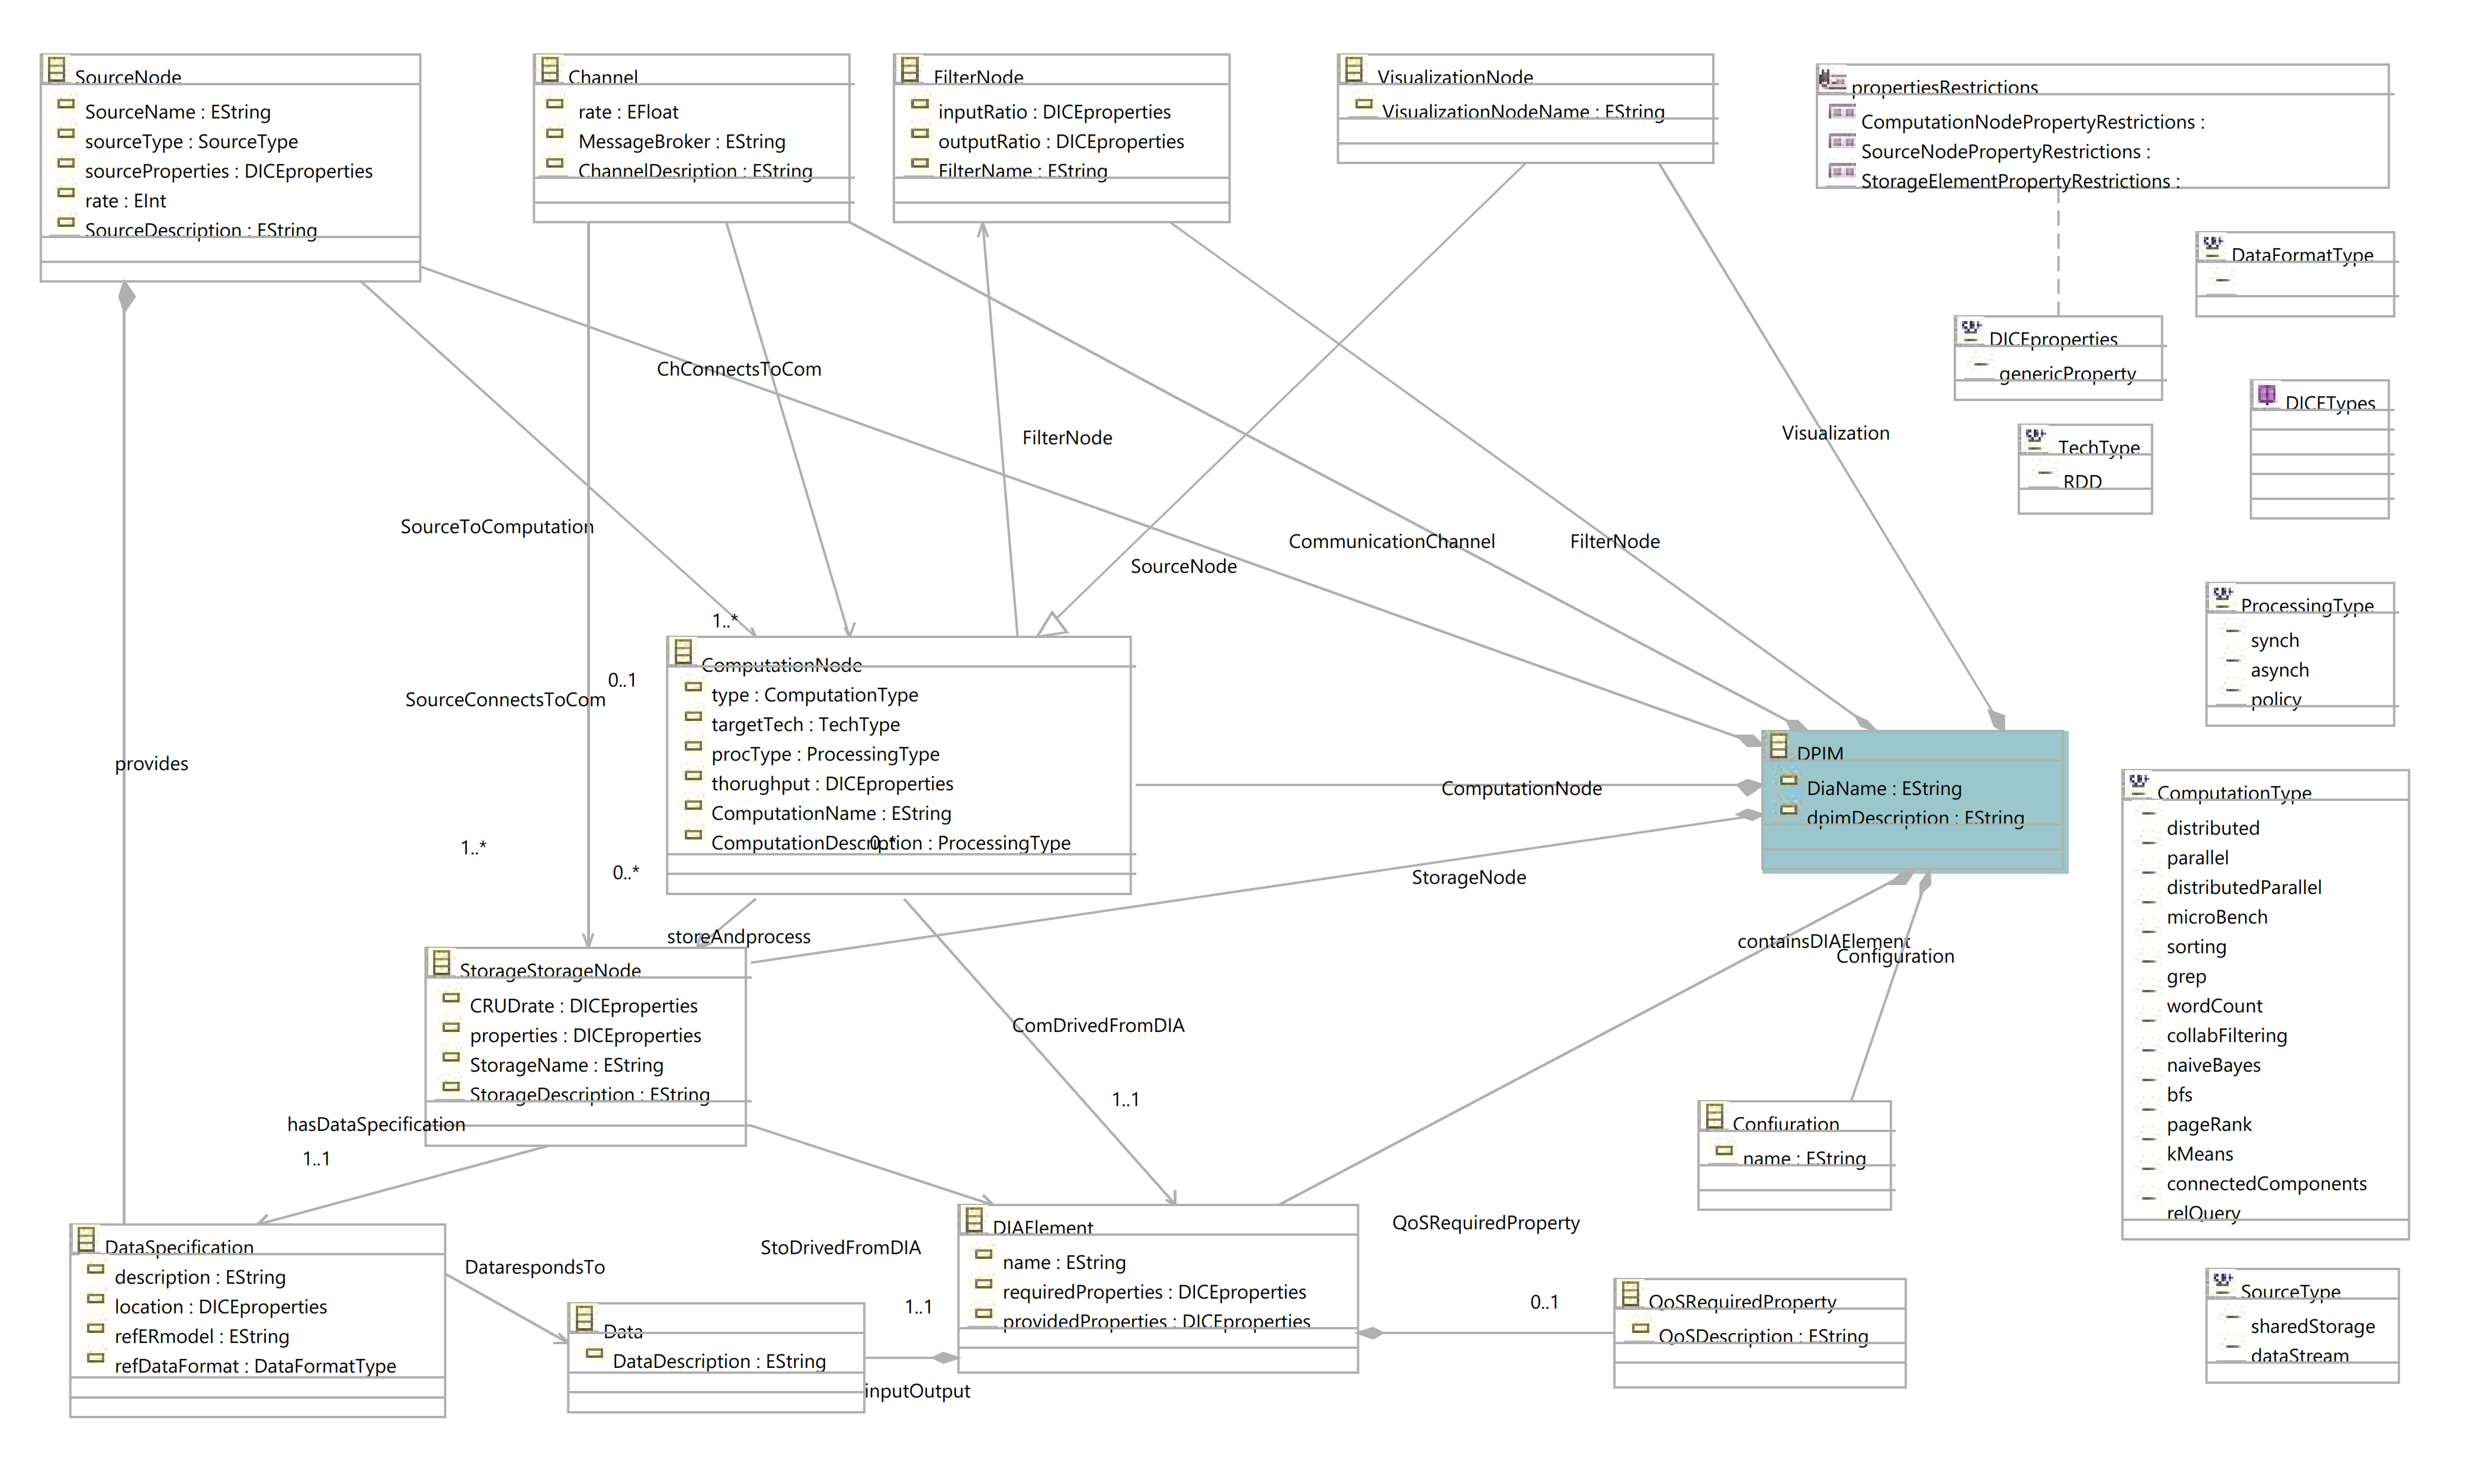
\includegraphics[width=\textwidth]{Images/11.png}
\caption{\label{fig:metamodel}DICE DPIM metamodel.}
\end{sidewaysfigure}

\begin{figure}
\centering
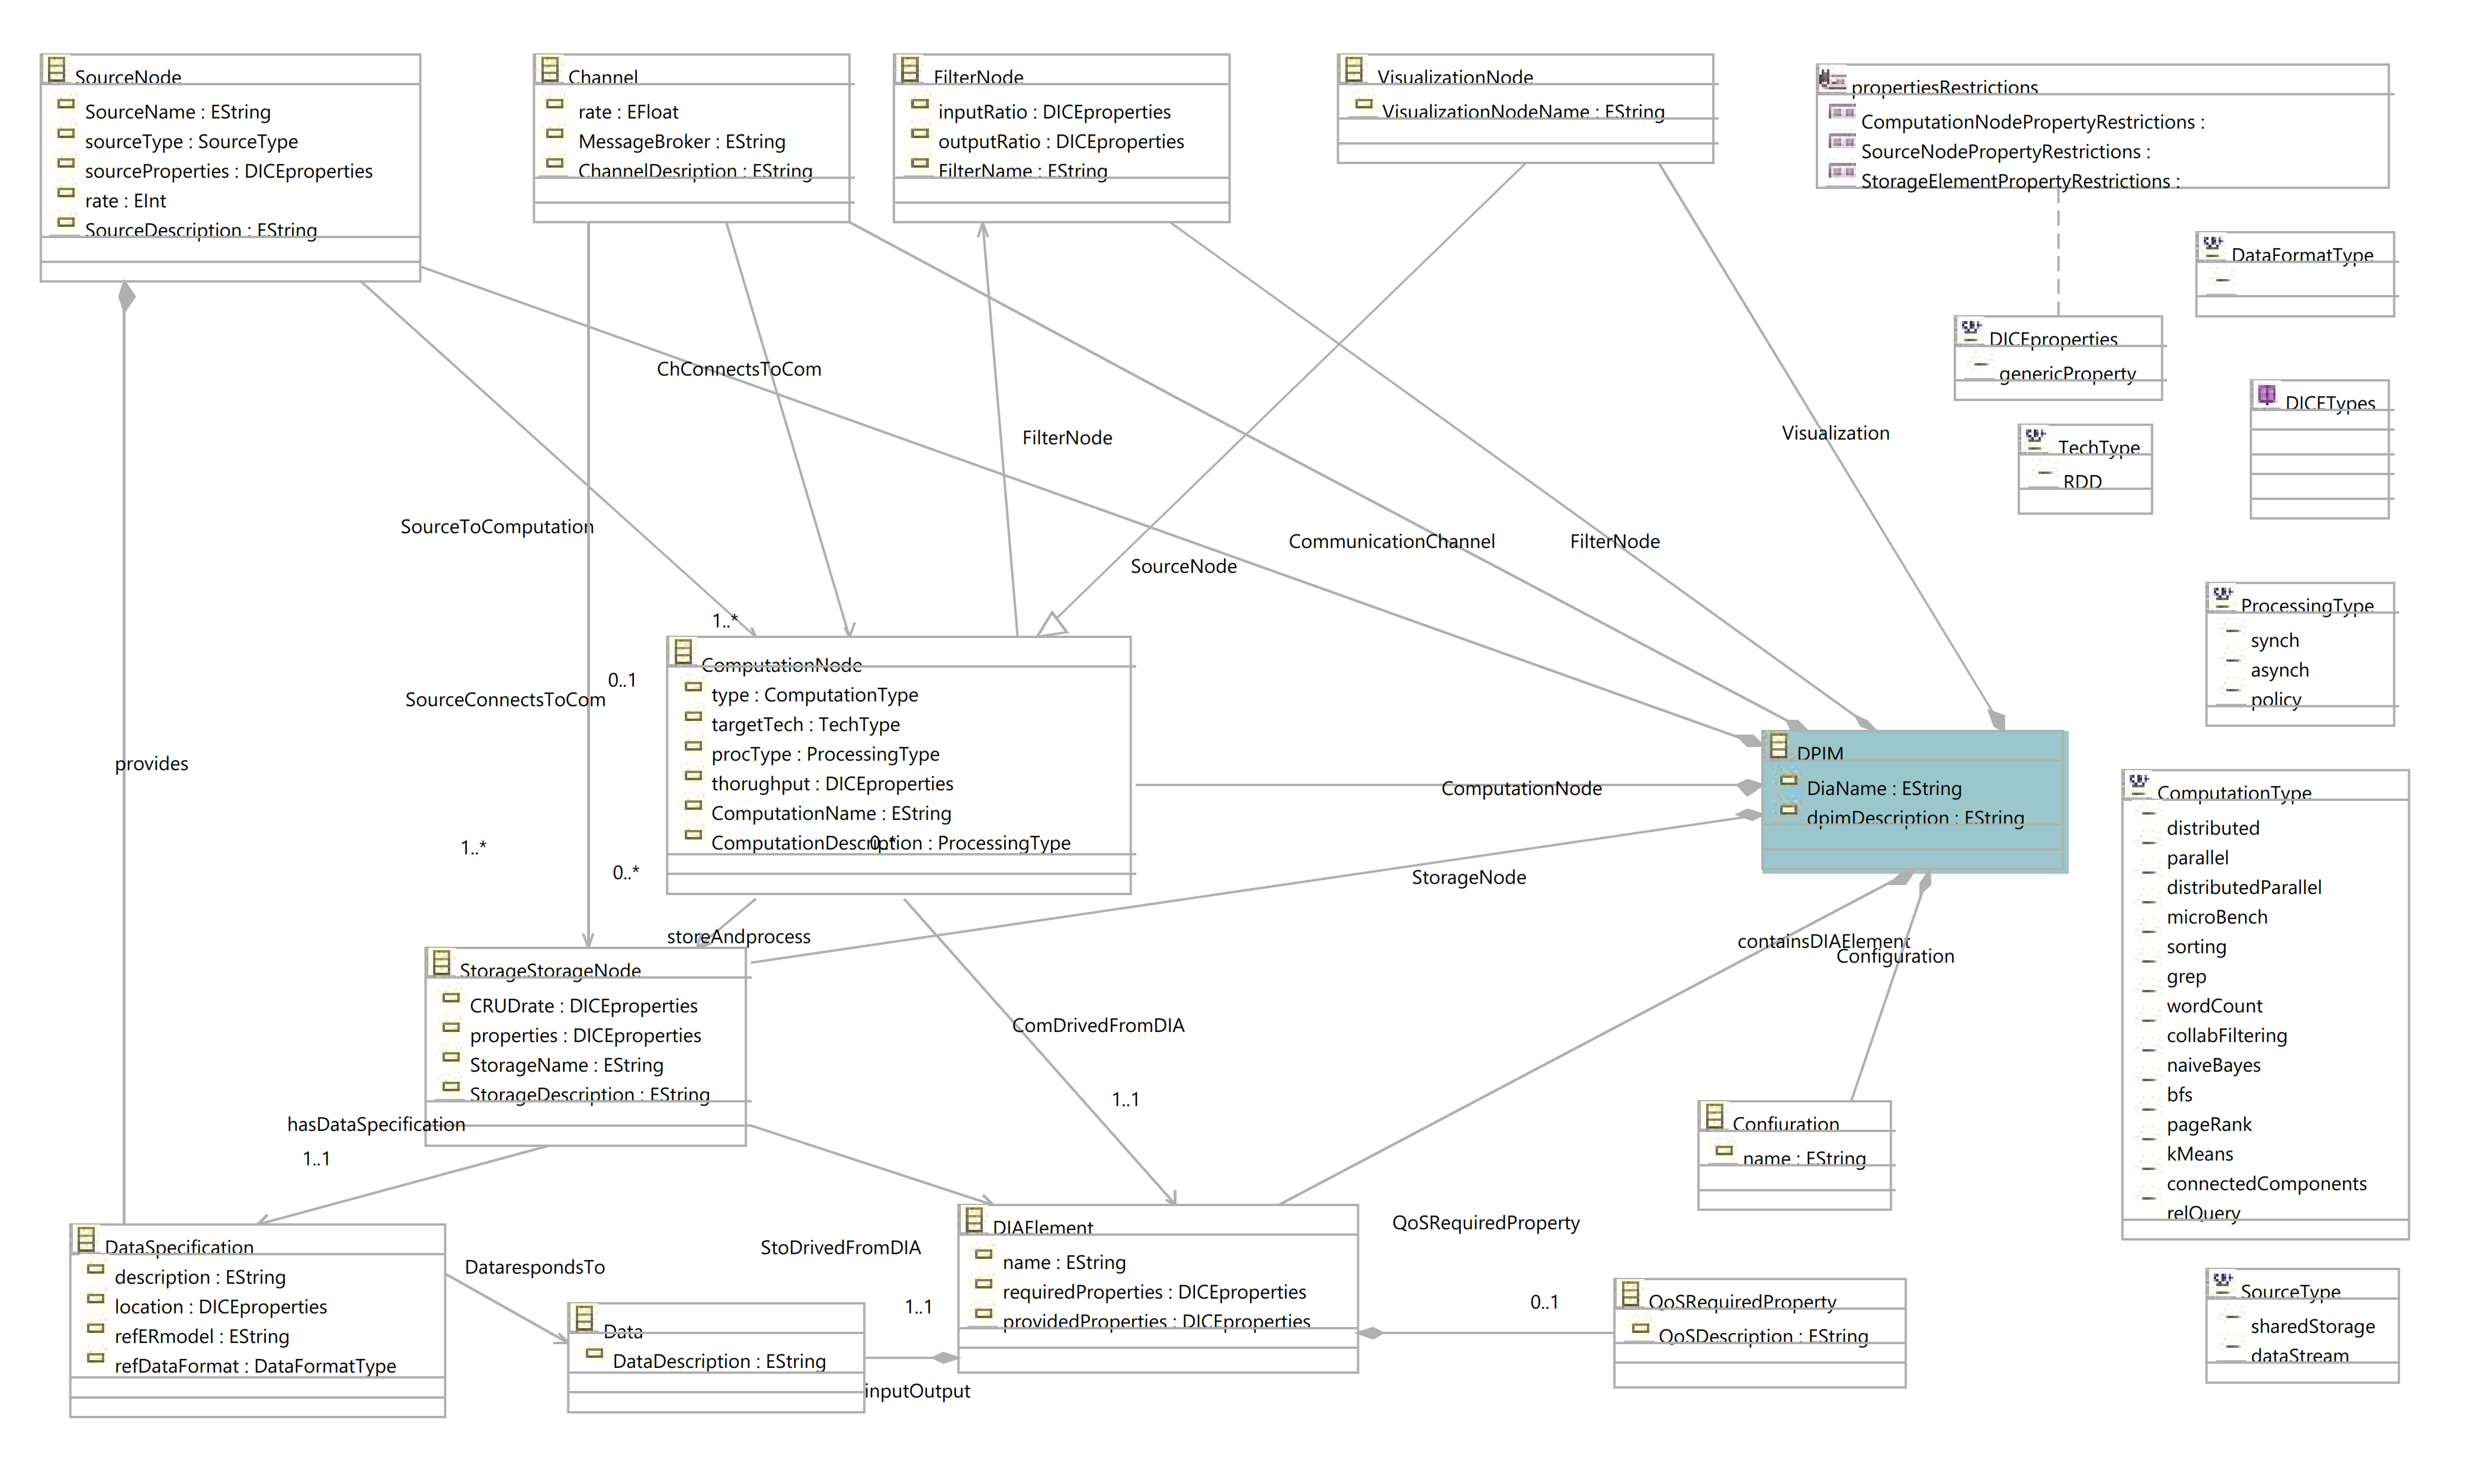
\includegraphics[width=\textwidth]{Images/11.png}
\caption{\label{fig:metamodel2}DICE DPIM metamodel in portrait form.}
\end{figure}

Here is the command to refer to another element (section, figure, table, ...) in the document: \emph{As discussed in Section~\ref{sect:overview} and as shown in Figure~\ref{fig:metamodel}, ...}. Here is how to introduce a bibliographic citation~\cite{DAM}. Bibliographic references should be included in a \texttt{.bib} file. 

Table generation is a bit complicated in Latex. You will soon become proficient, but to start you can rely on tools or external services. See for instance this \href{https://www.tablesgenerator.com}{https://www.tablesgenerator.com}. 


%------------------------------------------------------------------------------------------------------------------------------------------------
\clearpage
{\color{Blue}{\section{Specific Requirements}}}
\label{sect:requirements}
\subsection{External Interface Requirements}

\subsubsection{User Interfaces}
In order to access the Platform the crucial interface needed by the User is the one provided by a web browser. In fact, it is sufficient to reach the CKB's URL to start with log in or sign up operations, described in the scenarios, or, 
after authentication, interact with the Platform. The Platform software, in fact, is a Web App. Instead, to join a Battle a RMP link would be required.

\subsubsection{Hardware Interfaces}
Users have to provide themselves with a device able to access internet. It would be sufficient that it is equipped with a Wi-Fi and/or Ethernet interface. Of course would be crucial that it provides adequate components to allow Users 
to interact with the Platform, showing its interfaces and collecting inputs.

\subsubsection{Software Interfaces}
As defined above, a web browser is the only software needed to access the Platform. The interfaces that have to be supported are the ones defined by the Web Page rendering. About RMP, the Platform software run on the server would be 
equipped with appropriate interfaces to interact with the RMP provided by the Student or the Team in the steps described in previous sections of this document.
\subsubsection{Communication Interfaces}
Communication Interfaces needed are the one necessary to access the internet. So for the User, TCP and HTTP interfaces would be crucial to reach the server on which the Platform runs, while for the CKB's app it is fundamental to 
interact with RMP and with E-mail Provider. For this last communication the protocol that would be used is the SMTP, as for RMP the same ones described above for Client-Server interaction.

\newpage

\subsection{Functional Requirements}
Here follows a list of the Platform functional requirements:
\begin{enumerate}[label= \textbf{R\arabic*}]
    \item The Platform allows Users to sign in to the Platform itself either as Student either Educator.\label{req:reqSignin}
    \item The Platform allows Users to log in to the Platform. \label{req:reqLogin}
    \item The Platform shows Students the list of available Tournaments. \label{req:reqShowTournaments}
    \item The Platform allows registered Students to search for Tournaments. \label{req:reqSearchForTournament}
    \item The Platform allows registered Students to subscribe to Tournaments. \label{req:reqTournamentSubscription}
    \item The Platform allows registered Students to participate to Tournaments as a Team. \label{req:reqCreateTeam}
    \item The Platform allows registered Students to invite other Students to join a Team. \label{req:reqJoinTeam}
    \item The Platform allows registered Educators to create Tournaments. \label{req:reqCreateTournaments}
    \item The Platform allows registered Educators to create Battles in the context of a Tournament. \label{req:reqCreateBattle}
    \item The Platform allows registered Educators to manually assign scores to Teams in a context of a Battle in a Tournament managed by them. \label{req:reqManualEvalCode} 
    \item The Platform allows registered Educators to create Badges in the context of a Tournament. \label{req:reqCreateBadge}
    \item The Platform assigns a Battle Score to Teams' work. \label{req:reqEvaluateCode}
    \item The Platform provides a Teams' ranking based on the Tournament Score within a Tournament context. \label{req:reqRankingsUpdate}
    \item The Platform allows registered Educators to add other Educators to a Tournament. \label{req:reqJoinManagement}
    \item The Platform allows Users to search for other Users. \label{req:reqSearchForUsers}
    \item The Platform interacts properly with different RMPs to acquire the latest versions of code uploaded by related Teams. \label{req:reqPullRMP}
    \item The Platform awards Badges to deserving Students \label{req:reqAssignBadge}
\end{enumerate}

\newpage

\subsubsection{Use case diagrams}
\useSvgWithCaption{./Images/UML/useCaseDiagram/useCase1.svg}{0.92}{0.92}{Use case diagram of the login and the invitation}
\useSvgWithCaption{./Images/UML/useCaseDiagram/useCase2.svg}{0.95}{0.95}{Use case diagram of the Battle and the Tournament}

\newpage

\subsubsection{Use cases and associated sequence diagrams}
Here follow Use Case tables followed by respective sequence diagrams, to be followed with the "\nameref{uc:mapping}" Table, which shows the relationship between Scenarios, Use Cases and Requirements.
\paragraph{UC1 - User signs in to the Platform} \label{uc:uc1} 
\begin{center}
    \begin{tabu}{|X[.2]|X|} \hline \everyrow{\hline} 
        Name & User signs in to the Platform \\
        Actors & User \\ 
        Entry Condition & User has a valid e-mail address and valid RMP handle\\ 
        Event Flow & \begin{tabu}{X X[50]}
            1& At Homepage click on "Sign in" button\\
            2& System shows User the registration form\\
            3& User fills form with data, caring to choose his role accordingly\\
            4& User clicks on "Submit" button \\
            5& Platform saves submitted information\\
            6& Platform sends e-mail confirmation link to User\\
            7& User confirms e-mail by clicking confirmation e-mail\\
        \end{tabu} \\
        Exit Condition & User correctly registered in the Platform, User needs to login to use the Platform\\
        Exception & User provides an Email already in use.\\
        \specialReqLabel & - \\ 
    \end{tabu}
    \tableEntryByLabel{uc:uc1}
\end{center} 
"\nameref*{uc:uc1}" is a generalization of:\\
"\nameref{uc:uc1a}" and \\ "\nameref{uc:uc1b}".
\clearpage
\paragraph*{UC1a - Student signs in to the Platform} \label{uc:uc1a} 
\begin{center}
    \begin{tabu}{|X[.2]|X|} \hline \everyrow{\hline} 
        Name & Student signs in to the Platform \\ 
        Actors & Student \\ 
        Entry Condition & Same as \nameref{uc:uc1} \\ 
        Event Flow & Same as \nameref{uc:uc1} with exception of \newline \begin{tabu}{X X[50]}
            3& Student chooses Student role while filling in form\\
        \end{tabu} \\
        \exitCondLabel & Same as \nameref{uc:uc1}\\
        Exception & Same as \nameref{uc:uc1}\\
        \specialReqLabel & Same as \nameref{uc:uc1}\\ 
    \end{tabu}
    \tableEntryByLabel{uc:uc1a}
\end{center}
\useSvgWithCaption{./Images/UML/sequenceDiagram/sequenceDiagramUC1a.svg}{1.0}{1.0}{UC1, UC1a, Sequence Diagram - Student signs in to the Platform}
\clearpage

\paragraph*{UC1b - Educator signs in to the Platform} \label{uc:uc1b} 
\begin{center}
    \begin{tabu}{|X[.2]|X|} \hline \everyrow{\hline}
        Name & Educator signs in to the Platform \\ 
        Actors & Educator \\ 
        Entry Condition & Same as \nameref{uc:uc1} \\ 
        Event Flow & Same as \nameref{uc:uc1} with exception of \newline \begin{tabu}{X X[50]}
            3& Educator chooses Educator role while filling in form\\
        \end{tabu} \\
        Exit Condition & Same as \nameref{uc:uc1}\\
        Exception & Same as \nameref{uc:uc1}\\
        \specialReqLabel & Same as \nameref{uc:uc1}\\ 
    \end{tabu}
    \tableEntryByLabel{uc:uc1b}
\end{center}

\useSvgWithCaption{./Images/UML/sequenceDiagram/sequenceDiagramUC1b.svg}{1.0}{1.0}{UC1, UC1b Sequence Diagram - Educator signs in to the Platform}
\clearpage
\paragraph*{UC2}
\begin{center}
    \begin{tabu}{|X[.2]|X|} \hline \everyrow{\hline}
        Name & Student subscribes to tournament\\ 
        Actors & Student \\ 
        Entry Condition & - \\ 
        Event Flow & \begin{tabu}{X X[50]}
            1& Student logs in to the platform\\
            2& Student is in it's home page and is presented with a list of available tournaments\\
            3& Student scrolls through the list of available tournaments\\
            4& Student can ask to see more tournaments via the "See more" button\\
            5& Student clicks on tournament entry to see tournament details\\
            6& Student clicks again on tournament if not interested to hide details\\
            7& Student clicks on "subscribe" button to subscribe to tournament\\
            8& Platform registers tournament subscription\\
            9& Platform creates new team for that student\\
            10& Platform sends confirmation e-mail to student\\
            11& Platform gives visual feedback on web page of effective subscription\\
        \end{tabu} \\
        Exit Condition & Student is subscribed to tournament and knowing it\\
        Exception & Subscription deadline is passed, student cannot subscribe to tournament\\
        Special \newline Requirement & - \\ 
    \end{tabu}
\end{center}
\useSvgWithCaption{Images/UML/sequenceDiagram/sequenceDiagramStudentSubscribesToTournament.svg}{1.0}{1.0}{UC2 Sequence Diagram - Student subscribes to the tournament}
\clearpage
\paragraph*{UC3 - Student subscribes to Tournament} \label{uc:uc3}
\begin{center}
    \begin{tabu}{|X[.2]|X|} \hline \everyrow{\hline}
        Name & Student subscribes to Tournament\\ 
        Actors & Student \\ 
        Entry Condition & Tournament is in "ONLINE" state\\ 
        Event Flow & \begin{tabu}{X X[50]}
            1& Student logs in to the Platform\\
            2& Student is in its home page and is presented with a list of available Tournaments\\
            3& Student scrolls through the list of available Tournaments\\
            4& Student can ask to see more Tournaments via the "See more" button\\
            5& Student clicks on Tournament entry to see Tournament details\\
            6& Student clicks again on Tournament if not interested to hide details\\
            7& Student clicks on "subscribe" button to subscribe to Tournament\\
            8& Platform registers Tournament subscription\\
            9& Platform creates new Team for that Student\\
            10& Platform requests to insert the Team's name\\
            11& Student inserts the Team's name\\
            12& Platform sends confirmation e-mail to Student\\
            13& Platform gives visual feedback on web page of effective subscription\\
        \end{tabu} \\
        Exit Condition & Student is subscribed to Tournament and knows it\\
        Exception & Subscription deadline is passed, Student cannot subscribe to Tournament\\
        \specialReqLabel & - \\ 
    \end{tabu}
\end{center}
\useSvgWithCaption{Images/UML/sequenceDiagram/sequenceDiagramUC3.svg}{1.0}{1.0}{UC3 Sequence Diagram - Student subscribes to the Tournament}
\clearpage
\paragraph*{UC4 - User invites other user to collaborate} \label{uc:uc4}  
\begin{center}
    \begin{tabu}{|X[.2]|X|} \hline \everyrow{\hline}
        Name & User invites other user to collaborate \\ 
        Actors & Inviting user, invited user \\ 
        Entry Condition & Inviting user knows email of invited user \\ 
        Event Flow & \begin{tabu}{X X[50]}
            1& Inviting user clicks on "collaborate" button\\
            2& System shows inviting user a form to fill with the email of the user he wants to invite\\
            3& Inviting user clicks submit button\\
            4& System sends invite e-mail notification to invited user\\
            5& Invited user clicks on "Accept" button to accept invitation\\
            6& Invited user clicks on "Decline" button to decline invitation, or ignores it\\
        \end{tabu} \\
        Exit Condition & If invited user accepts invitation, invited user can collaborate with inviting one, else as nothing happened\\
        Exception & \begin{tabu}{X}
            Invited user e-mail address can be: non-existent, non-registered, of user of different role. In this case Inviting user get's notified of the error via e-mail.
        \end{tabu}  \\
        Special \newline Requirement & - \\ 
    \end{tabu}
\end{center}
"\nameref*{uc:uc4}" is a generalization of:\\
"\nameref{uc:uc4a}" and \\ "\nameref{uc:uc4b}".
\clearpage
\paragraph*{UC4a - Educator invites other educator to co-manage tournament} \label{uc:uc4a}
\begin{center}
    \begin{tabu}{|X[.2]|X|} \hline \everyrow{\hline}
        Name & Educator invites other educator to co-manage tournament\\ 
        Actors & Inviting educator, invited educator \\ 
        Entry Condition & Inviting educator is managing a tournament\\ 
        Event Flow & \begin{tabu}{X X[50]}
            1& Educator is in the managing page of the tournament\\
            & Event flow follows father's \nameref{uc:uc4} event flow
        \end{tabu} \\
        Exit Condition & Invited Educator can manage the tournament\\
        Exception & Same as \nameref{uc:uc4}\\
        Special \newline Requirement & - \\ 
    \end{tabu}
\end{center}
\useSvgWithCaption{Images/UML/sequenceDiagram/sequenceDiagramEducatorInvitesOtherEducator.svg}{1.0}{1.0}{UC4, UC4a Sequence Diagram - Educator invites educator to collaborate}
\clearpage
\paragraph*{UC4b - Student invites other student to participate in the tournament as a Team} \label{uc:uc4b}
\begin{center}
    \begin{tabu}{|X[.2]|X|} \hline \everyrow{\hline}
        Name & Student invites other student to participate in the tournament as a Team \\ 
        Actors & Inviting student, invited student\\ 
        Entry Condition & Inviting student is part of a team subscribed to a tournament \\ 
        Event Flow & \begin{tabu}{X X[50]}
            1& Student is in the tournament detail page\\
            & Follows follows father's \nameref{uc:uc4} event flow
        \end{tabu} \\
        Exit Condition & If invited student accepts invitation, invited user is part of inviting user's team\\
        Exception & Same as \nameref{uc:uc4}, with the verification of no participance to the Team in which he/she is invited or any other Team\\
        Special \newline Requirement & - \\ 
    \end{tabu}
\end{center}
\useSvgWithCaption{Images/UML/sequenceDiagram/sequenceDiagramStudentInvitesOtherStudent.svg}{1.0}{1.0}{UC4, UC4b Sequence Diagram - Student invites student to collaborate}
\clearpage
\begin{center}
    \begin{tabu}{|X[.2]|X|} \hline \everyrow{\hline}
        Name & Educator adds battle to tournament\\ 
        Actors & Educator \\ 
        Entry Condition & Educator has prepared: \newline 
        \begin{tabu}{X X[50]}
            -& Repository to be available for teams to fork\\
            -& Repository containing evaluation test suite\\
        \end{tabu} \newline 
        Tournament is not started\\ 
        Event Flow & \begin{tabu}{X X[50]}
            1& Educator is in tournament management page\\
            2& Educator clicks on "Add battle" button\\
            3& Platform shows a battle creation form\\
            4& Educator fills the form with link to repository in RMP\\
            5& Educator clicks on "Submit" button\\
            6& Platform registers battle addition to tournament\\
            7& Platfrom sends confirmation e-mail to Educator\\
        \end{tabu} \\
        Exit Condition & Platform is ready to test battles and code is available for students to fork\\
        Exception & Wrong  battle creation is discarded and Educator notified via e-mail of error\\
        Special Requirement & - \\ 
    \end{tabu}
\end{center}
\paragraph*{UC6 - Educator adds Battle to Tournament} \label{uc:uc6}
\begin{center}
    \begin{tabu}{|X[.2]|X|} \hline \everyrow{\hline}
        Name & Educator adds Battle to Tournament\\ 
        Actors & Educator \\ 
        Entry Condition & 
        Educator manages a Tournament \newline 
        Tournament is in "CREATED" state \newline 
        Educator has prepared: \newline 
        \begin{tabu}{X X[50]}
            -& Repository to be available for Teams to fork\\
            -& Repository containing evaluation test suite\\
        \end{tabu} \\
        Event Flow & \begin{tabu}{X X[50]}
            1& Educator is in Tournament management page\\
            2& Educator clicks on "Add Battle" button\\
            3& Platform shows a Battle creation form\\
            4& Educator fills the form with link to repository in RMP\\
            5& Educator clicks on "Submit" button\\
            6& Platform registers Battle addition to Tournament\\
            7& Platform sends confirmation e-mail to  the Educator\\
            8& Platform shows the new Battle's homepage to the Educator\\
        \end{tabu} \\
        Exit Condition & Platform is ready to test Battles and code is available for Students to fork\\
        Exception & - \\
        \specialReqLabel & - \\ 
    \end{tabu}
\end{center}
\useSvgWithCaption{Images/UML/sequenceDiagram/sequenceDiagramUC6.svg}{1.0}{1.0}{UC6 Sequence Diagram - Educator adds a Battle to the Tournament}
\clearpage
\paragraph*{UC7 - Educator creates Badge} \label{uc:uc7}
\begin{center}
    \begin{tabu}{|X[.2]|X|} \hline \everyrow{\hline}
        Name & Educator creates Badge \\ 
        Actors & Educator \\ 
        Entry Condition & Educator is managing a tournament \\ 
        Event Flow & \begin{tabu}{X X[50]}
            1& Educator is in tournament management page\\
            2& Educator clicks on "Add badge" button\\
            3& Platform shows badge creation form to educator\\
            4& Educator fills the form with badge image, description and test script\\
            5& Educator clicks on "Submit" button\\
            6& Platform checks badge test correctness\\
            7& Platform registers badge creation\\
            8& Platform sends a confirmation e-mail to educator\\
        \end{tabu} \\
        Exit Condition & Every user is able to see the existence of the badge in the tournament detail page\\
        Exception & If test script isn't correct, badge information is dropped and a notification e-mail is sent to the educator describing the issue\\
        Special \newline Requirement & - \\ 
    \end{tabu}
\end{center}
\useSvgWithCaption{Images/UML/sequenceDiagram/sequenceDiagramBadges.svg}{1.0}{1.0}{UC7 Sequence Diagram - Educator creates Badge}
\clearpage
\paragraph*{UC8 - Student gets awarded with Badge}   \label{uc:uc8}
\begin{center}
    \begin{tabu}{|X[.2]|X|} \hline \everyrow{\hline}
        Name & Student gets awarded with Badge\\ 
        Actors & Student \\ 
        Entry Condition & \begin{tabu}{@{}X}
            Student is part of a Team, and has contributed to Team's repository \\
            Tournament is in "OFFLINE" state\\
        \end{tabu} \\
        Event Flow & \begin{tabu}{X X[50]}
            1& System runs Badge tests on all repositories\\
            2& Badge tests give a list of RMP handles and e-mail addresses to which assign corresponding Badge\\
            3& System searches for corresponding accounts\\
            4& System assigns Badges to each User found\\
            5& System sends e-mail notification to chosen Students\\
        \end{tabu} \\
        Exit Condition & Random Platform User can see Badge in the specific Student profile page\\
        Exception & - \\
        \specialReqLabel & Commit User data is consistent with CKB Platform User data \\ 
    \end{tabu}
    \tableEntryByLabel{uc:uc8}
\end{center}
\useSvgWithCaption{Images/UML/sequenceDiagram/sequenceDiagramUC8.svg}{1.0}{1.0}{UC8 Sequence Diagram - Student gets awarded with Badge}
\clearpage
%\paragraph*{UC6 - Educator adds Battle to Tournament} \label{uc:uc6}
\begin{center}
    \begin{tabu}{|X[.2]|X|} \hline \everyrow{\hline}
        Name & Educator adds Battle to Tournament\\ 
        Actors & Educator \\ 
        Entry Condition & 
        Educator manages a Tournament \newline 
        Tournament is in "CREATED" state \newline 
        Educator has prepared: \newline 
        \begin{tabu}{X X[50]}
            -& Repository to be available for Teams to fork\\
            -& Repository containing evaluation test suite\\
        \end{tabu} \\
        Event Flow & \begin{tabu}{X X[50]}
            1& Educator is in Tournament management page\\
            2& Educator clicks on "Add Battle" button\\
            3& Platform shows a Battle creation form\\
            4& Educator fills the form with link to repository in RMP\\
            5& Educator clicks on "Submit" button\\
            6& Platform registers Battle addition to Tournament\\
            7& Platform sends confirmation e-mail to  the Educator\\
            8& Platform shows the new Battle's homepage to the Educator\\
        \end{tabu} \\
        Exit Condition & Platform is ready to test Battles and code is available for Students to fork\\
        Exception & - \\
        \specialReqLabel & - \\ 
    \end{tabu}
\end{center}
\useSvgWithCaption{Images/UML/sequenceDiagram/sequenceDiagramUC6.svg}{1.0}{1.0}{UC6 Sequence Diagram - Educator adds a Battle to the Tournament}
\clearpage
%\paragraph*{UC6 - Educator adds Battle to Tournament} \label{uc:uc6}
\begin{center}
    \begin{tabu}{|X[.2]|X|} \hline \everyrow{\hline}
        Name & Educator adds Battle to Tournament\\ 
        Actors & Educator \\ 
        Entry Condition & 
        Educator manages a Tournament \newline 
        Tournament is in "CREATED" state \newline 
        Educator has prepared: \newline 
        \begin{tabu}{X X[50]}
            -& Repository to be available for Teams to fork\\
            -& Repository containing evaluation test suite\\
        \end{tabu} \\
        Event Flow & \begin{tabu}{X X[50]}
            1& Educator is in Tournament management page\\
            2& Educator clicks on "Add Battle" button\\
            3& Platform shows a Battle creation form\\
            4& Educator fills the form with link to repository in RMP\\
            5& Educator clicks on "Submit" button\\
            6& Platform registers Battle addition to Tournament\\
            7& Platform sends confirmation e-mail to  the Educator\\
            8& Platform shows the new Battle's homepage to the Educator\\
        \end{tabu} \\
        Exit Condition & Platform is ready to test Battles and code is available for Students to fork\\
        Exception & - \\
        \specialReqLabel & - \\ 
    \end{tabu}
\end{center}
\useSvgWithCaption{Images/UML/sequenceDiagram/sequenceDiagramUC6.svg}{1.0}{1.0}{UC6 Sequence Diagram - Educator adds a Battle to the Tournament}
\clearpage
\subsection{Evaluation Requirements} \label{req:eval}
The Platform perform two types of evaluation: the Battle evaluation and the Badge Evaluation. 
The first one is performed automatically by the platform itself, is based on a testing environment set inside the Repository, useful for students to test their code before uploading it, that during evaluation gets overwritten with the code from the repository created by the educator to avoid cheating.
The second one is also performed automatically, but only at the end of a tournament. It is based on some assignment criteria that have to be standard to the platform, and well-defined for the educator to rightly assign the badges.

\subsection{Performance Requirements}
The Platform, that can be described as a Web App, has to be able to manage multiple Users requests, constantly update rankings for related Tournaments, perform tests on provided code and assign related Score, all at the same time. 

So, in order to satisfy all Requirements defined above, providing a good time response for each task, the Platform should have good time performance. Being a Web App, this implies a high concurrent programming implementation, to 
manage multiple requests at the same time, and a rapid related Data Storage System. 

\subsection{Design Constraints}

\subsubsection{Standard Compliance}
First of all, the Platform has to respect privacy standards, such as GDPR for EU countries or similar regulations, in order to protect personal information provided by Users when they sign in, their code and identity across the Web App.

It is also important to respect internet protocols standards and their rules, in order to make the app run and communicate properly. Other standards are related to UI accessibility features and servers' power consumption. 

\subsubsection{Hardware Limitations}
Hardware limitations in the RASD context are referred to User's machine capabilities and server's limits. 

In fact, the devices used by both Students and Educators are constrained by memory capacity, CPU capabilities and GPU computational power. The first is essential to memorize the file to upload in RMP, run the software to access internet
, to manage the Web App data itself and allow User to receive Emails. The second is fundamental to run the connection tasks and the site, receiving and elaborating inputs for the User and CKB's responses. Finally, GPU is essential to render UI and allows Users to read Emails via a proper Email Client App.\\
\\
 On server side, instead, is important for our App to have an organized storage to preserve all necessary data and enough computational power in our CPUs to manage multiple requests for each machine that composes CKB's server. 
 
In fact, to satisfy all possible inputs from all possible Users, formulating for each one a response, and meet requirements, is critical to have a multiple machine architecture on our servers. 

To complete, a multiple internet connection ports is fundamental, to make the Platform available on the internet and make it capable of comunication with Users, RMPs and Email Provider.

\subsection{Software System Attributes}

\subsubsection{Reliability}
The Platform described in this document should be an always available Web App. 

Downtimes are meant to be as less as possible, and the overall system, in order to prevent evaluation, ranking, registration, search problems, should be designed with robustness in mind and with built-in mechanisms to manage situations 
that could compromise information, materials and commands assigned to the Platform. All of this performed transparently to the Users as much as possible.

\subsubsection{Availability}
The Platform should be able as much as possible, 24/7, 365 days per year. 

The minimum availability rate should be 99\%. An inferior percentage could compromise educational activities potentially damaging Students.

\subsubsection{Security}
Both Users' devices and servers communications must always take place only via encrypted channels, using appropriate cryptographic protocols such as SSL. 

All operations and contributions to the Platform, except automated tasks performed on server side communicating with RMP and Email Provider, must be always explicitly approved by the Users.

\subsubsection{Maintainability}
In order to extend as much as possible the Platform's life cycle it should be designed with modularity in mind. 

This approach will guarantee the interchanging of old modules to update or to substitute, possibly maintaining the same interfaces and core functionalities, at minimum cost.

\subsubsection{Portability}
The Platform, intended to be build, would be used independently of the OS provided with the machine. 

In fact CKB can be accessed simply using just a web browser, on which maximum compatibility the developers should concentrate. 

On User side, it would be sufficient to guarantee portability to build the Web App using common internet standards and protocols to make it usable on any web browser.

About RPM portability, the Platform should be provided with the right interfaces and modules to communicate with the largest amount of RMPs available, in order to acquire and run code evaluating it.

%------------------------------------------------------------------------------------------------------------------------------------------------
\clearpage
{\color{Blue}{\section{Formal Analysis Using Alloy}}}
\label{sect:alloy}
\subsection{Signature}
abstract sig User {
    name: one Name,
    surname: one Surname,
    email: one Email,
    RMPHandle: one RMPHandle
}

sig Name{}
sig Surname{}
sig 

%------------------------------------------------------------------------------------------------------------------------------------------------
\clearpage
{\color{Blue}{\section{Effort Spent}}}
\label{sect:effort}
Provide here information about how much effort each group member spent in working at this document. We would appreciate details here.



%------------------------------------------------------------------------------------------------------------------------------------------------
\clearpage
\addcontentsline{toc}{section}{References}
\bibliographystyle{plain}
\bibliography{main_DD}
%------------------------------------------------------------------------------------------------------------------------------------------------




\end{document}
